\documentclass{article}
\usepackage{settings}
%to write english paragraph \selectlanguage{language}
%to write english inline \textenglish{...}

\title{winter24A}
\author{דורון שפיגל}
\date{18.05.24}

\begin{document}
\maketitle
\begin{Question}
נתונה מערכת של 2 רמות בטמפרטורה $T$. רמה ראשונה עם אנרגיה $\epsilon$ וניוון $1$ ורמה שנייה עם אנרגיה $2\epsilon$ וניוון $3$. מהי הטמפרטורה $T$  אם ידוע כי ההסתברות שהמערכת תהיה במצב אנרגיה $\epsilon$ שווה לרבע ההסתברות שהמערכת תהיה עם אנרגיה $2\epsilon$.
\end{Question}
\begin{Answer}
הנוסחה לחישוב פונקציית החלוקה $Z$ היא:
\begin{align}\label{פונקציית החלוקה}
    1&=\sum \limits^{}_{S}{P\left( s \right)}=\frac{1}{Z}\sum \limits^{}_{S}{e^{-\beta E\left( s \right)}}\\
    \rightarrow&Z\triangleq \sum \limits^{}_{S}{g(s)e^{\frac{-E\left( s \right)}{kT} }}=\sum \limits^{}_{S}{g(s)e^{-\beta E\left( s \right)}}
\end{align}
נסמן את הרמה הראשונה כ $s_{1}$ ואת הרמה השנייה כ $s_{2}$, נתון ש $P(s_{1})=\frac{1}{4}P(s_{2})$. מהנתון על הניוון של כל רמה, נסמן: $g(s_{1})=1$ ו $g(s_{2})=3$.\\
נכתוב את פונקציית החלוקה:
\begin{align*}
    Z&=g(s_{1})e^{-\beta E(s_{1})}+g(s_{2})e^{-\beta E(s_{2})}=e^{-\beta \epsilon}+3e^{-\beta 2\epsilon}\\
    P(s_{1})=\frac{1}{Z}e^{-\beta \epsilon}&=\frac{1}{4}P(s_{2})=\frac{3}{4Z}e^{-\beta 2\epsilon}\\
    \frac{1}{Z}e^{-\beta \epsilon}&=\frac{3}{4Z}e^{-\beta 2\epsilon}\\
    \frac{4}{3}e^{-\beta \epsilon}&=e^{-\beta 2\epsilon}\quad \backslash \cdot e^{2\beta \epsilon}\\
    \frac{4}{3}e^{\beta \epsilon}&=1\rightarrow e^{\beta \epsilon} = \frac{3}{4}\quad\backslash \ln\left(  \right)\\
    \beta \epsilon&=\ln\left( \frac{3}{4} \right)
\end{align*}
כידוע $\beta=\frac{1}{kT}$, לכן:
\begin{align*}
    \ln\left( \frac{3}{4} \right)&=\beta \epsilon\rightarrow \frac{\ln\left( \frac{3}{4} \right)}{\beta}=\epsilon\rightarrow \frac{1}{\beta}=\frac{\epsilon}{\ln\left( \frac{3}{4} \right)}\\
    \beta=\frac{1}{kT}\leftrightarrow \frac{1}{\beta}=kT\\
    kT&=\frac{\epsilon}{\ln\left( \frac{3}{4} \right)}\\
    T&=\frac{\epsilon}{k\ln\left( \frac{3}{4} \right)}
\end{align*}
\end{Answer}\newpage
\begin{Question}
נתונה מערכת מבודדת של שני גופים. גוף אחד עם קיבול חום $C_{1}=bT$ שהטמפרטורה שלו היא $T_{1}$ והשני בעל קיבול חום קבוע $C_{2}=aT$ שהטמפרטורה שלו היא $T_{2}$. נתון כי $T_{1}<T_{2}$. הגופים באים במגע. מה השינוי באנטרופיית המערכת עד ההגעה לשיווי משקל?
\end{Question}
\begin{Answer}
כיוון שגוף חם מעביר חום לגוף קר, בשיווי משקל המערכות יגיעו לטמפרטורה שנסמנה $T_{f}$ כך ש: $T_{1}<T_{f}<T_{2}$.
כמות האנרגיה שדרושה למערכת הראשונה כדי להגיע לטמפרטורה זאת שווה לכמות האנרגיה שהמערכת השנייה מאבדת, נמצא ביטוי לטמפרטורה זאת:
\begin{align*}
    Q_{1}&=C_{1}\Delta T=\int_{T_{1}}^{T_{f}}b\cdot T dT  = \frac{b (- T_{1}^{2} + T_{f}^{2})}{2}\\
    Q_{2}&=C_{2}\Delta T=\int_{T_{f}}^{T_{2}}a\cdot T dT = \frac{a (T_{2}^{2} - T_{f}^{2})}{2}\\
    Q_{1}&=Q_{2}\rightarrow \frac{b (- T_{1}^{2} + T_{f}^{2})}{2}=\frac{a (T_{2}^{2} - T_{f}^{2})}{2}\\
    T_{f}&=\sqrt{\frac{T_{1}^{2}b+T_{2}^{2}a}{a+b}}
\end{align*}
כעת, ידוע כי השינוי באנטרופית המערכת הוא סכום השינוי באנטרופיה של כל גוף: $\Delta S=\Delta S_{1}+\Delta S_{2}$. נחשב את השינוי באנטרופיה של כל גוף ונסכום:
\begin{align*}
    \Delta S_{1}&=\int_{T_{1}}^{T_{f}}\frac{C_{1}}{T}dT=\int_{T_{1}}^{T_{f}}\frac{bT}{T}dT = b (- T_{1} + T_{f})\\
    \Delta S_{2}&=\int_{T_{2}}^{T_{f}}\frac{C_{2}}{T}dT=\int_{T_{2}}^{T_{f}}\frac{aT}{T}dT = a (- T_{2} + T_{f})\\
    \Delta S&=b (- T_{1} + T_{f})+a (- T_{2} + T_{f})=T_{f}(a+b)-bT_{1}-aT_{2}\\
    \Delta S&=\sqrt{\frac{T_{1}^{2}b+T_{2}^{2}a}{a+b}}(a+b)-bT_{1}-aT_{2}
\end{align*}
\end{Answer}\newpage
\begin{Question}
נתונה מערכת המורכבת מ $N$ אתרים. לכל אתר יש 2 מצבים, \textbf{מצב מלא} שבו הוא מכיל חלקיק עם אנרגיה $\epsilon$ \textbf{ומצב ריק} שבו הוא לא מכיל חלקיק (אנרגיה 0). מה מספר האתרים המלאים הממוצע במערכת?\\
(תזכורת: פונקציית חלוקה כוללת של מערכת של $N$ חלקיקים ללא אינטרקציה היא $Z=Z_{1}^{N}$, כאשר $Z_{1}$ היא פונקציית חלוקה של חלקיק אחד).
\end{Question}
\begin{Answer}
פילוג ההסתברויות של מצבי האנרגיה באתר מסוים הן:
\begin{align*}
    P_{\text{full}}&=\frac{1}{Z}e^{-\beta \epsilon}\\
    P_{\text{empty}}&=\frac{1}{Z}e^{-\beta\cdot 0}=\frac{1}{Z}
\end{align*}
ופונקצית החלוקה עבור אתר מסוים היא:
\begin{align*}
    Z=Z_{\text{full}}+Z_{\text{empty}}=e^{-\beta \epsilon}+1
\end{align*}
לכן ההסתברות שאתר מסוים יהיה מלא היא:
\begin{align*}
    P_{\text{full}}=\frac{1}{Z}e^{-\beta \epsilon}=\frac{e^{-\beta \epsilon}}{e^{-\beta \epsilon}+1}
\end{align*}
לכן מספר האתרים המלאים הממוצע במערכת עם $N$ אתרים הוא:
$$n=N\cdot P_{\text{full}}=N\cdot \frac{e^{-\beta \epsilon}}{e^{-\beta \epsilon}+1}
$$
\end{Answer}\newpage
\begin{Question}
נתונה שכבת מתכת דו ממדית. כמו כן נתונה אנרגיית פרמי - עמוק בתוך הפס כך ש $E_{f}\gg kT$ וגם נתון יחס נפיצה פרבולי בפס. חשבו את האנרגיה הממוצעת של אלקטרון בודד בפס $E_{av}$.
\end{Question}
\begin{Answer}
    פונקצית המצבים עבור אלקטרונים ב $2D$ אינה תלויה באנרגיה, והיא:
    $$g(E)=\frac{m}{\pi \hbar^{2}}\equiv g_{0}$$
    ממהנחה ש $E_{f}\gg kT$ נוכל להניח שהתפלגות פרמי דיראק היא מדרגה:
    $$f_{FD}(E)=\begin{cases}
    1 & E<E_{f}\\
    0 & E>E_{f}
    \end{cases}$$
    צפיפות החלקיקים ליחידת אנרגיה ויחידת נפח היא:
    $$n(E)=g(E)f_{FD}(E)$$ מכפלה זאת נותנת את מספר המצבים באנרגיה $E$ שמאוכלסים על ידי אלקטרונים.
    ולכן, מספר החלקיקים במערכת הוא:
    $$N=\int_{-\infty}^{\infty}g(E)f_{FD}(E)dE=\int_{0}^{E_{f}}{g(E)dE}=\int_{0}^{E_{f}}g_{0}dE=E_{f}g_{0}$$
    עבור אינטגרל על $E\cdot n(E)$ אקבל את סכום התרומות שניתנות על ידי כל מצב $E$.
    $$E_{tot}=\int_{-\infty}^{\infty}E\cdot g(E)f_{FD}(E)dE=\int_{0}^{E_{f}}{E\cdot g_{0}dE}=\frac{1}{2}E_{f}^{2}g_{0}$$
    האנרגיה הממוצעת של אלקטרון בודד היא פשוט המנה של האנרגיה הכוללת על מספר החלקיקים:
    $$E_{av}=\frac{E_{tot}}{N}=\frac{\frac{1}{2}E_{f}^{2}g_{0}}{E_{f}g_{0}}=\frac{1}{2}E_{f}$$
\end{Answer}\newpage
\begin{Question}
נתונה מתכת עם ריכוז אלקטורנים $n$ וזמן ממוצע בין פיזורים $\tau$. לפי מודל דרודה, בשדה שתלוי בזמן $E\left( t \right)=E_{0}e^{i\omega t}$\\
הניחו $\to\infty$ אומר גדול מאוד ו $\to0$ אומר קטן מאוד, אבל הגדלים הם עדיין סופיים.\\
ההספק החשמלי יהיה מינימלי עבור?
$$\omega\to?\, \tau\to?\, n\to?$$
\end{Question}
\begin{Answer}
מוליכות המתכת היא:
$$\sigma\left( \omega \right)=\frac{ne^{2}\tau}{m\left( 1-i\omega\tau \right)}$$
כאשר $\omega\to\infty,\quad \tau\to\infty,\quad n\to 0$ נקבל שהמוליכות שואפת לאפס.\\
ההספק הנצרך על ידי המתכת הוא:
$$P\left( \omega \right)=\frac{1}{2}\sigma\left( \omega \right)\abs{E_{0}}^{2}$$
לכן נקבל שההספק הנצרך יהיה מינימלי עבור $\omega\to\infty,\quad \tau\to\infty,\quad n\to 0$.
\end{Answer}\newpage
\begin{Question}
נתון גביש דו-ממדי כאשר לפס האנרגיה שלו יש 2 נקודות מינימום, נקודה 1 ב $\vec{K_{1}}=\left( 0,0 \right)$ ונקודה 2 ב $\vec{K_{2}}=\left( k_{0},0 \right)$. נסמן את הפרש האנרגיה בין 2 נקודות המינימום ב $\Delta$, הפרש זה קטן מספיק כך כשמאכלסים מעט אלקטרונים סביב נקודה 1 אפשר לאכלס גם מעט אלקטרונים סביב נקודה 2. פס האנרגיה סביב כל אחת מהנקודות נתון לפי הפרבולות:
\begin{gather*}
    \epsilon_{1}\left( \vec{k} \right)=\frac{\hbar^{2}}{2m_{1}^{*}}\left( k_{x}^{2}+k_{y}^{2} \right)\\
    \epsilon_{2}\left( \vec{k} \right)=\frac{\hbar^{2}}{2m_{2}^{*}}\left( \left( k_{x}-k_{0} \right)^{2}+k_{y}^{2} \right)+\Delta,\quad \Delta>0
\end{gather*}
\begin{figure}[H]
\centering
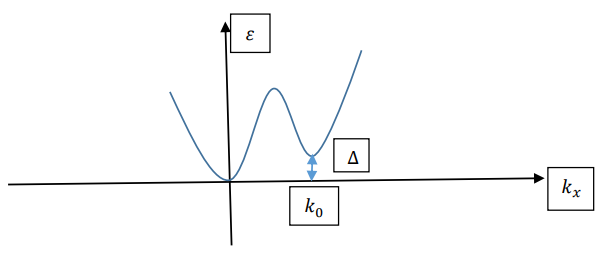
\includegraphics[width=0.9\textwidth]{images/Q6.png}
\caption{
בתמונה רואים חתך של הפס על ציר $k_{x}$ שבו מופיעות 2 נקודות המינימום (שימו לב שהמסות האפקטיביות שונות).}
%\label{}
\end{figure}
\begin{SubQuestion}
חשבו את צפיפות המצבים ליחידת שטח עבור כל אחת מהפרבולות.
\end{SubQuestion}
\begin{SubAnswer}
    יחס הנפיצה עבור חלקיקים בעלי מסה הוא:
    $$E=\frac{\hbar^{2}k^{2}}{2m}$$
    ראינו שפתרון המשוואה לצפיפות המצבים ליחידת אנרגיה וליחידת גודל, $g\left( E \right) = \od{G(E)}{E}$, במקרה ה $2D$ הוא:
    $$g\left( E \right)=\frac{m}{\pi \hbar^{2}}$$
    לכן:
    \begin{align*}
        \begin{cases}
            g_{1}\left( \epsilon \right)=\frac{m_{1}^{*}}{\pi \hbar^{2}}& \epsilon\geq0 \\
            g_{2}\left( \epsilon \right)=\frac{m_{2}^{*}}{\pi \hbar^{2}}     & \epsilon\geq\Delta 
        \end{cases}
    \end{align*}
\end{SubAnswer}
\begin{SubQuestion}
עבור $T=0$, מה התנאי על רמת פרמי כך שיש אכלוס של אלקטרונים בפרבולה 2? חשבו את צפיפות האלקטרונים בכל אחת משתי הפרבולות במקרה זה.
\end{SubQuestion}
\begin{SubAnswer}
כדי שיהיה אכלוס של אלקטרונים בפרבולה 2, יש צורך שהרמת פרמי תהיה גבוהה מהמינימום של פרבולה זאת:
$$\epsilon_{F}>\min{\left( \epsilon_{2} \right)}=\Delta$$
במקרה זה, פילוג פרמי דיראק הוא:
$$f_{FD}\left( \epsilon \right)=\begin{cases}
    1 & \epsilon<\Delta\\
    0 & \epsilon>\Delta
\end{cases}$$
מהנתון ש $\Delta$ מספיק קטן, עבור פרבולה 1, מספיק לדרוש עבורה:
$$f_{FD}\left( \epsilon_{1} \right)=\begin{cases}
    1 & \epsilon_{1}<\Delta\approx0\\
    0 & \epsilon_{1}>\Delta\approx0
\end{cases}$$
ולכן:
$$n_{1}=\int_{-\infty}^{\infty}g_{1}\left( \epsilon_{1} \right)f_{FD}\left( \epsilon_{1} \right)dE=\int_{0}^{\epsilon_{f}}\frac{m_{1}^{*}}{\pi \hbar^{2}}dE=\frac{m_{1}^{*}}{\pi \hbar^{2}}\epsilon_{f}
$$
ועבור פרבולה 2:
$$n_{2}=\int_{-\infty}^{\infty}g_{2}\left( \epsilon_{2} \right)f_{FD}\left( \epsilon_{2} \right)dE=\int_{\Delta}^{\epsilon_{f}}\frac{m_{2}^{*}}{\pi \hbar^{2}}dE=\frac{m_{2}^{*}}{\pi \hbar^{2}}\left( \epsilon_{f}-\Delta \right)
$$
\end{SubAnswer}
\begin{SubQuestion} 
האם יתכן ויהיו יותר אלקטרונים בפרבולה 2 מאשר בפרבולה 1 למרות שבפרבולה 2 האלקטרונים מאכלסים קטע יותר קטן על ציר האנרגיה?
\end{SubQuestion}
\begin{SubAnswer}   
%is it possible that there will be more electrons in parabola 2 than in parabola 1 even though in parabola 2 the electrons populate a smaller segment on the energy axis?
%yes, because the density of states in parabola 2 is higher than in parabola 1
כן, כי צפיפות המצבים בפרבולה 2 גבוהה יותר מאשר בפרבולה 1. עבור $m_{2}^{*}>m_{1}^{*}$. כאשר צפיפות המצבים גבוהה יותר, יש יותר אלקטרונים בכל קטע אנרגיה.
\end{SubAnswer} 
\end{Question}













\end{document}